\chapter{Linear Systems and Matrices}
In this chapter we'll assume that you are familiar with the basics of linear algebra.
Hence, you can use the appropriate linked text from Section \ref{pref:resources} for any
necessary explanation on these problems.  I highly suggest you use your notes from when
you first saw linear algebra.  We will begin here with a few of the basic definitions and
we will recap some of the basics from systems of equations, row reduction, linear
combinations, and matrix operations.  I highly suggest that you \underline{{\bf PUT YOUR
CALCULATOR DOWN}} and get used to doing all of these techniques by hand.  There is a time
and place for technology and for the most part this chapter is not it.




\section{Matrix Operations and Definitions}
\begin{definition}[Size of a Matrix]
    If $A$ is a matrix with $m$ rows and $n$ columns then we say that $A$ has
    size (or
    dimensions) $m \times n$.
\end{definition}

\begin{definition}[Equality of Matrices]
    Two matrices are equal if their corresponding entries are equal. Matrices can only be
    equal if the sizes are equal.
\end{definition}

\begin{definition}[Addition and Subtraction of Matrices] 
    Matrix addition and subtraction and done by regular addition and subtraction on the
    corresponding entries. Matrix addition and subtraction can only be performed on
    matrices of the same size.
\end{definition}

\begin{definition}[Scalar Multiplication]
    If $A$ is a matrix then $cA$ is a scalar multiple of the matrix.  Multiplying a matrix
    by a scalar multiplies every entry by the scalar.
\end{definition}

\begin{definition}[Transposition of a Matrix] 
    If $A$ is a matrix then $A^T$
    is the transpose of the matrix found by interchanging
    the rows and columns of $A$. If $A$ is $m \times n$ then $A^T$
    is $n \times m$.
\end{definition}
    
\begin{definition}
    If $A$ is an $m \times n$ matrix and $B$ is an $n \times p$ matrix then the product of
    $A$ and $B$ is $C = AB$ where:
    \begin{itemize}
        \item The size of $AB$ is $m \times p$.  The number of columns in $A$ must be the
            same as the number of rows of $B$.
        \item The entry in row $i$ and column $j$ of $C = AB$ is
            \[ c_{ij} = a_{i1} b_{1j} + a_{i2}b_{2j} + \cdots + a_{in}b_{nj} =
            \sum_{k=1}^n a_{ik}b_{kj}.\]
    \end{itemize}
    It is very important to note that in general $AB \ne BA$.
\end{definition}

\begin{problem}
    Consider the matrices $A$ and $B$.  Find the products $AB$ and $BA$ if they exist.
    \[ A = \begin{pmatrix} 1 & 2 & -3 \\ 2 & 0 & 1 \end{pmatrix} \qquad B =
    \begin{pmatrix} 5 & -2 \\ -1 & 0 \\ 1 & 3 \end{pmatrix} \]
\end{problem}
\solution{
    \[ AB = \begin{pmatrix} 0 & -11 \\ 11 & -1 \end{pmatrix} \qquad BA = \begin{pmatrix} 1
        & 10 & -17 \\ -1 & -2 & 3 \\ 7 & 2 & 0 \end{pmatrix} \]
}


\begin{problem}
    Consider the matrices below.
    \[ A = \begin{pmatrix} 2 & -1 & 4 \\ 3 & 0 & 1 \end{pmatrix} \quad B = \begin{pmatrix}
            2 & 1 \\ 0 & -3 \\ 4 & -1 \end{pmatrix} \quad C = \begin{pmatrix} 0 & -1 \\ 3
            & 2 \\ -3 & 1 \end{pmatrix} \quad \bx = \begin{pmatrix} 1 \\ 3 \\ -2
    \end{pmatrix} \]
    \begin{enumerate}
        \item[(a)] Determine which products are possible:
            \[ AB, \quad AC, \quad A\bx, \quad BA, \quad CA, \quad \bx A, \quad BC,
            \quad B \bx, \quad CB, \quad C\bx. \]
            For each of the products that is possible find the size of the result.
        \item[(b)] Write the product $AB$ and the product $BA$.  Does $AB = BA$?
    \end{enumerate}
\end{problem}
\solution{
The matrix products that exist are: $AB: 2 \times 2$, $AC: 2 \times 2$, $A \bx: 2 \times
1$, $BA: 3 \times 3$, $CA: 3 \times 3$.  None of the rest exist. \\
As expected, $AB \ne BA$.
}


\begin{problem}
    Compute the product $Ab$ for 
    \[ A = \begin{pmatrix} 2 & 1 \\ 3 & 2 \end{pmatrix} \quad b = \begin{pmatrix} a \\ b
        \end{pmatrix} \]
\end{problem}
\solution{
}


\newpage\section{Gaussian Elimination: Reduced Row Echelon Form}
Solving systems of equations is one of the most essential applications of linear algebra.
It is expected that you have experience solving systems with row reduction so as such we
will cover it quickly in this section.

\begin{problem}
    Consider the system of equations:
    \[ \left\{ \begin{array}{cc} -x_1 + x_2 - x_3 &= -6 \\ x_1 + x_3 &= 15 \\ 2x_1 - x_2 +
        x_3 &= 9 \end{array} \right. \]
    We want to solve this system of equations using Gaussian elimination (row reduction).
    We will do so using the following steps.
    \begin{enumerate}
        \item[(a)] For the sake of practice let's first write this system as a matrix
            equation of the form $A \bx = \bb$.  What are $A$, $\bx$, and $\bb$?
\solution{
    \[ \begin{pmatrix} -1 & 1 & -1 \\ 1 & 0 & 1 \\ 2 & -1 & 1 \end{pmatrix}
            \begin{pmatrix} x_1 \\ x_2 \\ x_3 \end{pmatrix} = \begin{pmatrix} -6 \\ 15 \\
                    9 \end{pmatrix} \]
}
        \item[(b)] Next write the system as an {\it augmented matrix}.  
            \[ \left( \begin{array}{ccc|c}
                    \underline{\hspace{0.25in}} & \underline{\hspace{0.25in}}
                    &\underline{\hspace{0.25in}} &\underline{\hspace{0.25in}} \\
                    \underline{\hspace{0.25in}} & \underline{\hspace{0.25in}}
                    &\underline{\hspace{0.25in}} &\underline{\hspace{0.25in}} \\
                    \underline{\hspace{0.25in}} & \underline{\hspace{0.25in}}
                    &\underline{\hspace{0.25in}} &\underline{\hspace{0.25in}} \end{array}
            \right) \]
            \solution{
                \[ \left( \begin{array}{ccc|c} -1 & 1 & -1 & -6 \\ 1 & 0 & 1 & 15 \\ 2 &
                        -1 & 1 & 9 \end{array} \right) \]
            }
        \item[(c)] Our goal is to transform the augmented matrix $\left( A | \bb \right)$
            to the matrix $\left( I | \bx \right)$ using only the following operations:
            \begin{itemize}
                \item multiply one row by a scalar quantity
                \item add a multiple of one row to another row
                \item interchange two rows
            \end{itemize}
            Discuss why we are allowed to use these operations.
            \solution{These {\it moves} are legal since each row represents a linear
            equation and we are simply manipulating the equations while making sure that
        the equal sign remains true.}
        \item[(d)] Starting with the top left corner of the augmented matrix,
            systematically row reduce the matrix to the form $\left( I | \bx \right)$.
            \solution{
                \[ \left( \begin{array}{ccc|c} -1 & 1 & -1 & -6 \\ 1 & 0 & 1 & 15 \\ 2 &
                        -1 & 1 & 9 \end{array} \right)
                    \to \left( \begin{array}{ccc|c} 1 & -1 & 1 & 6 \\ 0 & 1 & 0 & 9 \\ 2 &
                        -1 & 1 & 9 \end{array} \right)
                    \to \left( \begin{array}{ccc|c} 1 & -1 & 1 & 6 \\ 0 & 1 & 0 & 9 \\ 0 &
                        1 & -1 & -3 \end{array} \right)
                        \]
                \[ 
                    \to \left( \begin{array}{ccc|c} 1 & 0 & 1 & 15 \\ 0 & 1 & 0 & 9 \\ 0 &
                        1 & -1 & -3 \end{array} \right)
                    \to \left( \begin{array}{ccc|c} 1 & 0 & 1 & 15 \\ 0 & 1 & 0 & 9 \\ 0 &
                        0 & -1 & -12 \end{array} \right)
                    \to \left( \begin{array}{ccc|c} 1 & 0 & 0 & 3 \\ 0 & 1 & 0 & 9 \\ 0 &
                        0 & 1 & 12 \end{array} \right)
                        \]
            }
        \item[(e)] Once you have the row reduced matrix interpret your result.
            \solution{
Our row reduction gives us 
\[ \begin{pmatrix} x_1 \\ x_2 \\ x_3 \end{pmatrix} = \begin{pmatrix} 3 \\ 9 \\ 12
    \end{pmatrix} \]
            }
    \end{enumerate}
\end{problem}

\begin{technique}[Practical Tips for Gaussian Elimination]
    When performing Gaussian Elimination you should keep the following in mind:
    \begin{itemize}
        \item First try to get a 1 in the upper left-hand corner of the augmented matrix.
        \item Next, use the new first row to eliminate all of the non-zero entries in the first
            column. By the
            time you're done with this you should have a column with a 1 on top and zeros below.
        \item Next get a 1 in row 2 column 2.
        \item Use your new second row to eliminate all of the non-zero entries in the second
            column.
        \item Proceed in a similar fashion until you have reached the final row
    \end{itemize}
\end{technique}

\begin{example}
    Let's row reduce an augmented matrix.  Pay particular attention to the systematic way
    that we work toward getting the identity matrix on the left-hand side of the augmented
    matrix.
        \begin{flalign*}
            \left( \begin{array}{cc|c} 2 & -2 & 6 \\ 2 & 1 & 0 \end{array} \right) &\xrightarrow{R_1 \gets (1/2)R_1} \left( \begin{array}{cc|c} 1 &
            -1 & 3 \\ 2 & 1 & 0 \end{array} \right) \\
            &\xrightarrow{R_2 \gets R_2-2R_1} \left( \begin{array}{cc|c} 1 &
                -1 & 3 \\ 0 & 3 & -6 \end{array} \right)\\
            &\xrightarrow{R_2 \gets (1/3)R_2} \left( \begin{array}{cc|c} 1 &
            -1 & 3 \\ 0 & 1 & -2 \end{array} \right) \\
            &\xrightarrow{R_1 \gets R_2+R_1} \left( \begin{array}{cc|c} 1 &
            0 & 1 \\ 0 & 1 & -2 \end{array} \right)
        \end{flalign*}
    Notice further that at each step we indicate which row operations were done.  Finally
    notice that there are no equal signs since the matrices that you create at each step
    are definitely not equal; they are called ``row equivalent''.
\end{example}
I
leave it to you to make yourself familiar with examples of Gaussian Elimination from other
texts (see the linked materials in Section \ref{pref:resources} of these notes).

\begin{problem}
    Consider the following three systems of equations and their row reduced forms.
    Describe their solution sets geometrically.  If the system has a solution then give
    it.  If the system has no solution then explain why.  If the system has infinitely
    many solutions then give them all in a parameterized form.
    \begin{flalign*}
        & \text{System \#1: } \quad \left( \begin{array}{cc|c} 1 & -1 & 3 \\ 2 & 1 & 0
        \end{array} \right) \to \cdots \to \left( \begin{array}{cc|c} 1 & 0 & 1 \\ 0 & 1 &
            -2 \end{array} \right) \\
        & \text{System \#2: } \quad \left( \begin{array}{cc|c} 1 & -1 & 3 \\ -1 & 1 & 0
        \end{array} \right) \to \cdots \to \left( \begin{array}{cc|c} 1 & -1 & 3 \\ 0 & 0 &
            3 \end{array} \right) \\
        & \text{System \#3: } \quad \left( \begin{array}{cc|c} 1 & -1 & 3 \\ -1 & 1 & -3
        \end{array} \right) \to \cdots \to \left( \begin{array}{cc|c} 1 & -1 & 3 \\ 0 & 0 &
            0 \end{array} \right) \\
    \end{flalign*}
\end{problem}
\solution{
System \#1 has one unique solution $x_1 = 1, x_2 = -2$.  System \#2 has no solution.
System \#3 has infinitely many solutions $x_1 = 3 + t, x_2 = t$ for $t \in \mathbb{R}$.
}

% 
% \begin{problem}
%     \begin{itemize}
%             \input{ClickerQuestions/LA.00.01.020}
%     \end{itemize}
%     Verify your answer with matrices.
% \end{problem}
% \solution{
% 2
% }
% 
% \begin{problem}
%     \begin{itemize}
%             \input{ClickerQuestions/LA.00.01.023}
%     \end{itemize}
%     \begin{center}
%         \includegraphics[width=0.75\columnwidth]{ClickerQuestions/LA_00_01_023.eps}
%     \end{center}
% \end{problem}
% \solution{
% b
% }

% 

\begin{problem}
    Create $3\times 3$ systems of equations that have
    \begin{enumerate}
        \item[(a)] exactly 1 solution
        \item[(b)] no solutions
        \item[(c)] infinitely many solutions
    \end{enumerate}
\end{problem}

\begin{problem}
    What is the value of $k$ so that the linear system represented by the following matrix
    would have infinitely many solutions?
    \[ \left( \begin{array}{cc|c} 2 & 6 & 8 \\ 1 & k & 4 \end{array} \right) \]
    Choose from the following choices:\\
    (a) $k=1$, \quad (b) $k=2$, \quad (c) $k=3$, \quad (d) $k=4$, \quad (e) not possible,
    \quad (f) there are infnitely many ways to do this
\end{problem}
\solution{$k=3$}

% 
% \begin{problem}
%     \begin{itemize}
%             \input{ClickerQuestions/LA.00.03.040}
%     \end{itemize}
% \end{problem}
% \solution{
% 3
% }
% 

\begin{problem}
We have a system of three linear equations with two unknowns as plotted in the graph

    \begin{minipage}{0.45\columnwidth}
        How many solutions does the system have?  Choose from the following: \\
        (a) 0, \quad (b) 1, \quad (c) 2, \quad (d) 3, \quad (e) infinite
    \end{minipage}
    \begin{minipage}{0.5\columnwidth}
        \begin{center}
            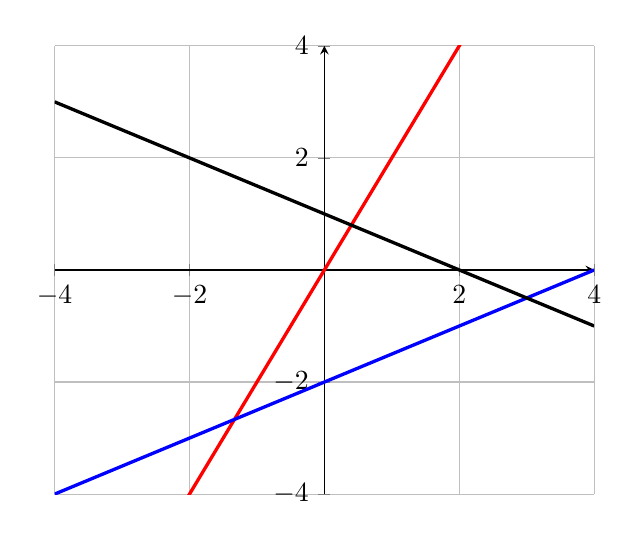
\begin{tikzpicture}
                \begin{axis}[axis lines=center, grid, domain=-4:4, xmin=-4, xmax=4,
                    ymin=-4, ymax=4]
                    \addplot[red, very thick] {2*x};
                    \addplot[blue, very thick] {0.5*x-2};
                    \addplot[black, very thick] {-0.5*x+1};
                \end{axis}
            \end{tikzpicture}
        \end{center}
    \end{minipage}

\end{problem}
\solution{No solution}

\begin{problem}
We have a system of two linear equations with two unknowns as plotted in the graph

    \begin{minipage}{0.45\columnwidth}
        How many solutions does the system have?  Choose from the following: \\
        (a) 0, \quad (b) 1, \quad (c) 2, \quad (d) 3, \quad (e) infinite
    \end{minipage}
    \begin{minipage}{0.5\columnwidth}
        \begin{center}
            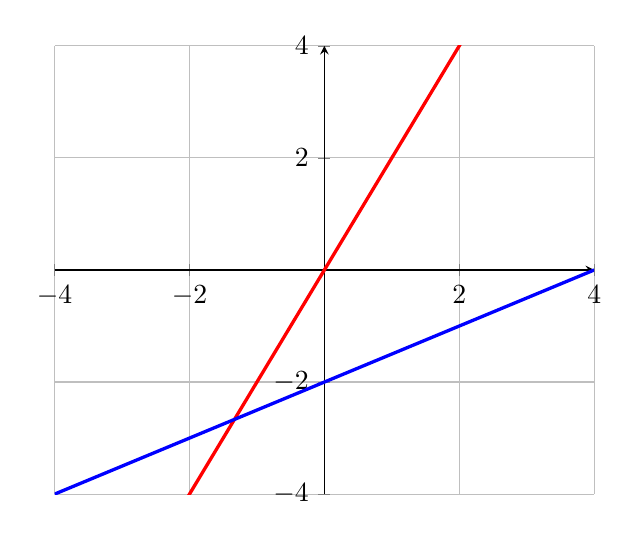
\begin{tikzpicture}
                \begin{axis}[axis lines=center, grid, domain=-4:4, xmin=-4, xmax=4,
                    ymin=-4, ymax=4]
                    \addplot[red, very thick] {2*x};
                    \addplot[blue, very thick] {0.5*x-2};
                \end{axis}
            \end{tikzpicture}
        \end{center}
    \end{minipage}

\end{problem}
\solution{One Solution}


\begin{problem}
We have a system of two linear equations with two unknowns as plotted in the graph

    \begin{minipage}{0.45\columnwidth}
        How many solutions does the system have?  Choose from the following: \\
        (a) 0, \quad (b) 1, \quad (c) 2, \quad (d) 3, \quad (e) infinite
    \end{minipage}
    \begin{minipage}{0.5\columnwidth}
        \begin{center}
            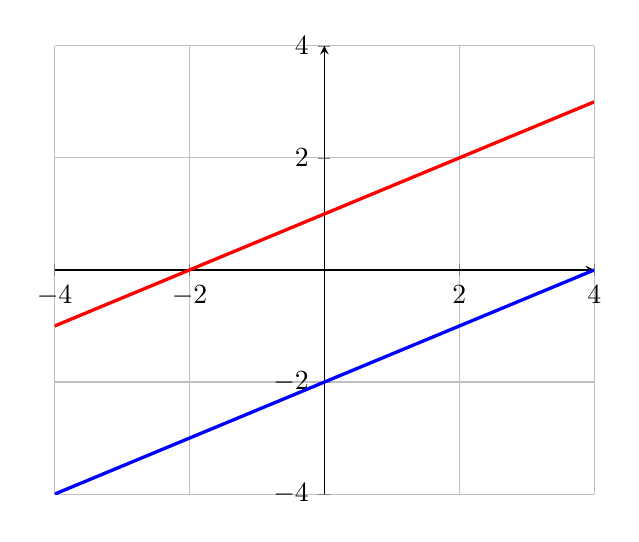
\begin{tikzpicture}
                \begin{axis}[axis lines=center, grid, domain=-4:4, xmin=-4, xmax=4,
                    ymin=-4, ymax=4]
                    \addplot[red, very thick] {0.5*x+1};
                    \addplot[blue, very thick] {0.5*x-2};
                \end{axis}
            \end{tikzpicture}
        \end{center}
    \end{minipage}

\end{problem}
\solution{No Solutions}


% \begin{problem}
%     \begin{itemize}
%             \input{ClickerQuestions/LA.00.01.035}
%     \end{itemize}
%     \begin{center}
%         \includegraphics[width=0.60\columnwidth]{ClickerQuestions/LA_00_01_035.eps}
%     \end{center}
% \end{problem}
% \solution{
% 1 - no solution
% }


\begin{problem}
    The following system has infinitely many solutions.  Write an equation that expresses
    all of them in a parameterized form.
    \begin{flalign*}
        x+y&=2 \\
        -3x-3y&=-6\\
        2x+2y&=4
    \end{flalign*}
\end{problem}
\solution{
    $x=t$ and $y=2-t$ for all $t \in \mathbb{R}$.
}

% \begin{problem}
%     \begin{itemize}
%             \input{ClickerQuestions/LA.00.01.054}
%     \end{itemize}
% \end{problem}
% \solution{
% 2
% }
% 
% 
% \begin{problem}
%     \begin{itemize}
%             \input{ClickerQuestions/LA.00.01.086}
%     \end{itemize}
% \end{problem}
% \solution{
% 
% }
% 
% 
% 
% 

\begin{problem}
    A system of 8 linear equations and 6 variables could not have exactly
    \underline{\hspace{0.5in}} solution(s).  \\ (a) 0, \quad (b) 1, \quad (c) infinite, \quad
    (d) more than one of these is possible, \quad (e) all of these are possible
\end{problem}
\solution{
Infinitely many solution or no solutions
}
% \begin{problem}
%     \begin{itemize}
%             \input{ClickerQuestions/LA.00.01.100}
%     \end{itemize}
% \end{problem}
% \solution{
% 4
% }
% 
% 
% \begin{problem}
%     \begin{itemize}
%             \input{ClickerQuestions/LA.00.02.020}
%     \end{itemize}
% \end{problem}
% 
% 
\begin{problem}
    What is the solution to the system of equations represented by this augmented matrix?
    \[ \left( \begin{array}{ccc|c} 1 & 0 & 3 & 2 \\ 0 & 1 & 2 & 3 \\ 0 & 0 & 0 & 0
        \end{array} \right) \]
    Choose from:
    \begin{enumerate}
        \item[(a)] $x=2, y=3, z=4$
        \item[(b)] $x=-2, y=1, z=1$
        \item[(c)] There are infinitely many solutions
        \item[(d)] There is no solution
        \item[(e)] We can't tell without having the system of equations
    \end{enumerate}
    (If there are infinitely many solutions then write expression for all of them)
\end{problem}
\solution{
There are infinitely many
\[ \begin{pmatrix} x \\ y \\ z \end{pmatrix} = \begin{pmatrix} 2 \\ 3 \\ 0 \end{pmatrix} +
        \begin{pmatrix} -3 \\ -2 \\ 1 \end{pmatrix} t \quad t \in \mathbb{R} \]
}

% \begin{problem}
%     \begin{itemize}
%             \input{ClickerQuestions/LA.00.02.060}
%     \end{itemize}
%     If there are infinitely many solutions find them all.
% \end{problem}
% \solution{
% 3
% }
% 
% 
% \begin{problem}
%     \begin{itemize}
%             \input{ClickerQuestions/LA.00.03.047}
%     \end{itemize}
% \end{problem}
% 
% 

\begin{problem}
    Solve the system of equations
    \begin{flalign*}
        x+2y+z &= 0 \\
        x + 3y - 2z &= 0 
    \end{flalign*}
\end{problem}
\solution{
    \[ \begin{pmatrix} x \\ y \\ z \end{pmatrix} = \begin{pmatrix} -7 \\ 3 \\ 1
        \end{pmatrix} t \quad t \in \mathbb{R} \]
}

% \begin{problem}
%     \begin{itemize}
%             \input{ClickerQuestions/LA.00.04.020}
%     \end{itemize}
% \end{problem}
% \solution{
%     1
% }
% 
% 

\begin{problem}
    Let $R$ be the reduced row echelon form of matrix $A$.  True or False: the solutions
    to $R \bx = \bo$ are the same as the solutions to $A \bx = \bo$.
\end{problem}
\solution{True}

\begin{problem}
    Let $R$ be the reduced row echelon form of matrix $A$.  True or False: the solutions
    to $R \bx = \bb$ are the same as the solutions to $A \bx = \bb$.
\end{problem}
\solution{False}



% \begin{problem}
%     \begin{itemize}
%             \input{ClickerQuestions/LA.00.04.070}
%     \end{itemize}
% \end{problem}
% \solution{
% 1
% }
% 
% \begin{problem}
%     \begin{itemize}
%             \input{ClickerQuestions/LA.00.04.080}
%     \end{itemize}
% \end{problem}
% \solution{
% 3
% }
% 
% 
% 
% 

\newpage\section{Linear Combinations}
One of the most beautiful parts of linear algebra is the richness of the structure of
matrices. As you already know, every system of linear equations can be written several
different ways: as a system, as a matrix equation, as a vector equation, or as an
augmented system. 

\begin{example}
    For example, we can write the system of equations
    \begin{flalign*}
        2x_1 + 3x_2 &= 5 \\ 
        4x_1 - 6x_2 &= 6
    \end{flalign*}
    equivalently in the following ways:
    \begin{flalign*}
        & \text{Algebraic System: } \quad \begin{array}{cc} 
            2x_1 + 3x_2 &= 5 \\ 
            4x_1 - 6x_2 &= 6 \end{array} \\
            & \text{Matrix Equation: } \quad \begin{pmatrix} 2 & 3 \\ 4 & -6 \end{pmatrix}
                \begin{pmatrix} x_1 \\ x_2 \end{pmatrix} = \begin{pmatrix} 5 \\ 6 \end{pmatrix} \\
                    & \text{Vector Equation: } \quad x_1 \begin{pmatrix} 2 \\ 4 \end{pmatrix} + x_2
                        \begin{pmatrix} 3 \\ -6 \end{pmatrix} = \begin{pmatrix} 5 \\ 6 \end{pmatrix} \\
                            & \text{Augmented System: } \quad \left( \begin{array}{cc|c} 2 & 3 & 5 \\ 4 & -6 & 6
                            \end{array} \right).
                        \end{flalign*}
                    \end{example}
In this section we’ll look in particular at the vector equation.  Hiding behind a vector
equation is one of the most fundamental ideas behind all of linear algebra: the linear
combination.  The ``vector equation'' above really says ``some amount of $\begin{pmatrix}
    2\\4\end{pmatrix}$ plus some amount of $\begin{pmatrix} 3\\-6\end{pmatrix}$ gives
$\begin{pmatrix} 5\\6\end{pmatrix}$ and our job is to find the amounts that make the
equality true.''  More generally, the vector equation is saying that $\begin{pmatrix}
    5\\6\end{pmatrix}$ is a linear combination of the other two vectors.


Let's first start with a simple exercise.

\begin{problem}
    Write the system of equations as a vector equation.
    \begin{flalign*}
        x_1 + 3x_2 - 5x_3 &= 9 \\
        -x_1 + x_2  &= -3 \\
        7x_1 + 2x_3 &= -\pi 
    \end{flalign*}
\end{problem}
\solution{
    \[ x_1 \begin{pmatrix} 1 \\-1\\7\end{pmatrix} + x_2 \begin{pmatrix}
            3\\1\\0\end{pmatrix} + x_3 \begin{pmatrix}-5\\0\\2\end{pmatrix} =
    \begin{pmatrix} 9\\-3\\-\pi\end{pmatrix} \]
}

\begin{definition}[Linear Combination]
    Let $\bv_1, \bv_2, \bv_3, \ldots, \bv_p$ be vectors in $n$-dimensional space and let
    $c_1, c_2, c_3, \ldots, c_p$ be scalar quantities.  The vector $\bu$ defined by
    \[ \bu = c_1 \bv_1 + c_2 \bv_2 + c_3 \bv_3 + \cdots + c_p \bv_p = \sum_{j=1}^p c_j
    \bv_j \]
    is called a linear combination of the vectors $\bv_1, \bv_2, \bv_3, \ldots, \bv_p$
    with weights $c_1, c_2, c_3, \ldots, c_p$.
\end{definition}


\begin{problem}
    Open the GeoGebra applet:
    \href{https://www.geogebra.org/m/WShmQvQU}{www.geogebra.org/m/WShmQvQU} in a browser window.
    \begin{enumerate}
        \item[(a)] Move the vectors $\bu$ and $\bv$ to $\bu = \begin{pmatrix} 1 \\
                2\end{pmatrix}$ and $\bv = \begin{pmatrix} 2\\-1\end{pmatrix}$.
        \item[(b)] Describe all of the possible vectors $\bw = c_1 \bu + c_2 \bv$ if $c_1
            = 0$
        \item[(c)] Describe all of the possible vectors $\bw = c_1 \bu + c_2 \bv$ if $c_2
            = 0$
        \item[(d)] Is it possible to find $c_1$ and $c_2$ such that $\bw = \begin{pmatrix} -6
                \\ 0.5 \end{pmatrix}$.  If so, what are $c_1$ and $c_2$.
    \end{enumerate}
\end{problem}
\solution{
    \begin{enumerate}
        \item[(a)] -
        \item[(b)] This will be a line pointing in the same direction of $\bv$
        \item[(c)] This will be a line pointing in the same direction of $\bw$
        \item[(d)] For this problem we want to find $c_1$ and $c_2$ such that $\bw = c_1
            \bu + c_2 \bv$.
            \begin{flalign*}
                &c_1 \bu + c_2 \bv = \bw \\
                \implies& \left( \begin{array}{cc|c} 1 & 2 & -6 \\ 2 & -1 & 0.5 \end{array}
                    \right) \to \left( \begin{array}{cc|c} 1 & 2 & -6 \\ 0 & -5 & 12.5 \end{array}
                    \right) \to \left( \begin{array}{cc|c} 1 & 2 & -6 \\ 0 & 1 & -2.5 \end{array}
                    \right)  \to \left( \begin{array}{cc|c} 1 & 0 & -1 \\ 0 & 1 & -2.5 \end{array}
                    \right) 
            \end{flalign*}
            so if we take $c_1 = -1$ and $c_2 = -2.5$ we get $\bw = - \bu - 2.5 \bv$
    \end{enumerate}
}

% 

\begin{problem}
    Write $\bu = \begin{pmatrix} -5 \\ 3 \\ 16 \end{pmatrix}$ as a linear combination of
        $\bv = \begin{pmatrix} 1 \\ -1 \\ 4 \end{pmatrix}$ and $\bw = \begin{pmatrix} -3
            \\ 2 \\ 6 \end{pmatrix}$
\end{problem}
\solution{
    $\bu$ cannot be written as a linear combination of these vectors.
}

% \begin{problem}
%     \begin{itemize}
%             \input{ClickerQuestions/LA.00.05.020}
%     \end{itemize}
% \end{problem}
% \solution{
% 5
% }
% 
% 



\newpage\section{Inverses and Determinants}
Division is always a bit of a touchy subject. In the real numbers division is well defined
except when the denominator is zero. The same story is true in the rational numbers: a
fraction divided by a fraction is another fraction so long as the divisor is not zero.
What if we wanted to stay only in the integers? Can we divide two integers and get another
integer? Of course you can always divide by 1, but in most other cases division will move
you into the rational numbers. Hence, division on the integers doesn't really make
sense.  Mathematically speaking we say that the integers are not closed under addition.

Similarly, if we try to define division on matrices we run into trouble. What does it mean
to divide by a matrix? In general, that phrase is meaningless! Let's expand our view a
bit.

When considering the operation of addition, we call $0$ the additive identity and we call
$(−a)$ the
additive inverse of $a$ since $a + (-a) = 0$. When considering multiplication, we call $1$ the
multiplicative
identity and $1/a$ is the multiplicative inverse of $a$ (when $a\ne 0$) since $a \cdot
\frac{1}{a} = 1$.  To define the matrix inverses of a square matrix $A$ we seek the same
thing:  find matrix $B$ such
that $AB = I$ and $BA = I$. Where $I$ is the identity matrix which is the multiplicative
identity for matrices.

\begin{problem}
    \begin{enumerate}
        \item[(a)] Consider the matrix $A = \begin{pmatrix}
                1&2\\-4&-6\end{pmatrix}$ and the vector $\bb = \begin{pmatrix}
                5\\-16\end{pmatrix}$.
            Find the vector $\bx$ such that $A\bx = \bb$ by hand using row reduction.  
        \item[(b)] Consider the matrix $A = \begin{pmatrix} 1 & 2 \\ -4 & -6
            \end{pmatrix}$.  Find a matrix $B$ such that $AB = I$ and $BA = I$.  Use what
            you did in part (a) to help set up the problem. \\ (You may recall some sort
            of ``shortcut'' that involves switching and negating some matrix entries \dots
            you are forbidden to use this shortcut!)
    \end{enumerate}
\end{problem}
\solution{
Augment with the identity and row reduce.
\[ \left( \begin{array}{cc|cc} 1 & 2 & 1 & 0 \\ -4 & -6 & 0 & 1 \end{array} \right) \to 
\left( \begin{array}{cc|cc} 1 & 2 & 1 & 0 \\ 0 & 2 & 4 & 1 \end{array} \right) \to 
\left( \begin{array}{cc|cc} 1 & 2 & 1 & 0 \\ 0 & 1 & 2 & 1/2 \end{array} \right) \to 
\left( \begin{array}{cc|cc} 1 & 0 & -3 & 1 \\ 0 & 1 & 2 & 1/2 \end{array} \right) 
\]
}

\begin{problem}
    \begin{enumerate}
        \item[(a)] True or False: If $AB = I$ and $BA = I$ then $A$ is the inverse of $B$
            and $B$ is the inverse of $A$. \solution{True}
        \item[(b)] True or False: If $A\bx = \bb$ and $A$ has an inverse then $\bx =
            A^{-1} \bb$.\solution{True}
        \item[(c)] True or False: If $A \bx = \bb$ and $A^{-1}$ exists then to find $\bx$ we can augment $A$
            with $\bb$ and row reduce.  That is, $\begin{pmatrix} A & | & \bb
            \end{pmatrix} \to \cdots \to \begin{pmatrix} I & | & \bx
            \end{pmatrix}$.\solution{True}
        \item[(c)] True or False: If $A \bx = \bb$ then $A = \bb \bx^{-1}$.
            \solution{False}
        \item[(d)] True or False: If $AB = I$ then we can find $B$ by augmenting $A$ with $I$ and row
            reducing?  That is, $\begin{pmatrix} A & | & I \end{pmatrix} \to \cdots \to
            \begin{pmatrix} I & | & B \end{pmatrix}$. \solution{True}
    \end{enumerate}
\end{problem}

\begin{technique}[Finding Matrix Inverses]
    If $A$ is a square matrix of size $n \times n$ then if $A^{-1}$ exists we know that
    $AA^{-1} = I$.  Therefore, to find $A^{-1}$ we augment $A$ with $I$ and row reduce.
    That is, $\begin{pmatrix} A & | & I \end{pmatrix} \to \cdots \to \begin{pmatrix} I & |
        & B \end{pmatrix}$

    If $A^{-1}$ does not exist then we will be unable to row reduce to the identity.
\end{technique}
\solution{
    Augment with the identity and row reduce.
}

\begin{problem}
    Give an example of a non zero $2 \times 2$ matrix that does not have an inverse.
\end{problem}
\solution{
    \[ A = \begin{pmatrix} 1 & 0 \\ 0 & 0 \end{pmatrix} \]
}

\begin{problem}
    Which of the following matrices does not have an inverse?\\
%     \begin{enumerate}
        (a) $\begin{pmatrix} 1 & 2 \\ 3 & 4 \end{pmatrix}$, \quad (b)
        $\begin{pmatrix} 2 & 2 \\ 4 & 4 \end{pmatrix}$, \quad (c)
        $\begin{pmatrix} -1 & 0 \\ 0 & 3 \end{pmatrix}$, \quad (d)
        $\begin{pmatrix} 0 & 4 \\ 2 & 0 \end{pmatrix}$, \quad (e)
        More than one of these does not have an inverse, \quad (f)
        All have inverses
%     \end{enumerate}
\end{problem}
\solution{
(b)
}

% \begin{problem}
%     \begin{itemize}
%             \input{ClickerQuestions/LA.00.09.010}
%     \end{itemize}
% \end{problem}
% \solution{
% 2
% }

\begin{problem}
    When we put a matrix $A$ into row reduced echelon form, we get the following matrix.
    What does this mean?
    \[ A \to \begin{pmatrix} 1 & 2 \\ 0 & 0 \end{pmatrix} \]
    \begin{enumerate}
        \item[(a)] Matrix $A$ has no inverse
        \item[(b)] The matrix we have found is the inverse of $A$
        \item[(c)] Matrix $A$ has an inverse but this isn't it
        \item[(d)] This tells us nothing about whether $A$ has an inverse.
    \end{enumerate}
\end{problem}
\solution{(a)}

% \begin{problem}
%     \begin{itemize}
%             \input{ClickerQuestions/LA.00.09.020}
%     \end{itemize}
% \end{problem}
% \solution{
% 1
% }


% \begin{problem}
%     
% \end{problem}
%  
% \begin{problem}
%     \begin{itemize}
%             \input{ClickerQuestions/LA.00.09.025}
%     \end{itemize}
% \end{problem}
% \solution{
% 4
% }
% 

\begin{problem}
    True or False: Suppose that $A$, $B$, and $C$ are square matrices and $CA = B$ and $A$
    is invertible.  This means that $C = A^{-1} B$.
\end{problem}
\solution{False}

% \begin{problem}
%     \begin{itemize}
%             \input{ClickerQuestions/LA.00.09.050}
%     \end{itemize}
% \end{problem}
% \solution{
% 3
% }
% 

\begin{problem}
    $A$ and $B$ are invertible matrices.  If $AB = C$ then what is the inverse of $C$? \\
    (a) $C^{-1} = A^{-1} B^{-1}$, \quad 
    (b) $C^{-1} = B^{-1} A^{-1}$, \quad 
    (c) $C^{-1} = A B^{-1}$, \quad 
    (d) $C^{-1} = B A^{-1}$, \quad \\
    (e) More than one of these is true, \quad \\ (f) Just because $A$ and $B$ have inverses
    this doesn't mean that $C$ has an inverse
\end{problem}
\solution{
(b)
}

% \begin{problem}
%     \begin{itemize}
%             \input{ClickerQuestions/LA.00.09.070}
%     \end{itemize}
% \end{problem}
% \solution{
% 2
% }

\begin{problem}
The {\it trick} that you might recall for $2\times 2$ inverses is
\[ \begin{pmatrix} a & b \\ c & d \end{pmatrix}^{-1} = \frac{1}{ad-bc} \begin{pmatrix} d &
    -b \\ -c & a \end{pmatrix}. \]
Prove that this {\it trick} works by row reducing the system
\[ \left( \begin{array}{cc|cc} a & b & 1 & 0 \\ c & d & 0 & 1 \end{array} \right). \]
\end{problem}

In the demoninator of the equation
\[ \begin{pmatrix} a & b \\ c & d \end{pmatrix}^{-1} = \frac{1}{ad-bc} \begin{pmatrix} d &
    -b \\ -c & a \end{pmatrix}. \]
you find the expression $ad-bd$.  For a $2 \times 2$ matrix this is called the
determinant.  Clearly from this formula for the inverse of a $2\times 2$ matrix if the
determinant is zero then the inverse does not exist.  What we'll find is that this is not
unique to $2\time 2$ matrices.

\begin{definition}[$2\times 2$ Determinant]
    Let $A = \begin{pmatrix} a & b \\ c & d \end{pmatrix}$.  The determinant of $A$ is 
    \[ \det(A) = ad - bc. \]
\end{definition}

\begin{problem}
    What is the determinant of $A = \begin{pmatrix} 4 & -1 \\ -2 & 1 \end{pmatrix}$?
\end{problem}
\solution{
$\det(A) = 4-2=2$
}
%
\begin{problem}
    Find the value of $k$ so that the matrix $A$ is not invertible.
    \[ A = \begin{pmatrix} 2 & 4 \\ 3 & k \end{pmatrix} \]
\end{problem}

\begin{problem}
    Given the matrix 
    \[ B = \begin{pmatrix} 2-x & 1 \\ 4 & 2-x \end{pmatrix} \]
    find all of the values of $x$ that are solutions to the equation $\det(B) = 0$.
\end{problem}


\begin{problem}\label{prob:det_3}
    Now consider the matrix 
    \[ A = \begin{pmatrix} 1 & 5 & 3 \\ 2 & 4 & -1 \\ 0 & -2 & 0 \end{pmatrix}. \]
    \begin{itemize}
        \item Cross out row 1 and column 1. Call the remaining $2 \times 2$ matrix
            $A_{11}$.
        \item Cross out row 1 and column 2. Call the remaining $2 \times 2$ matrix
            $A_{12}$.
        \item Cross out row 1 and column 3. Call the remaining $2 \times 2$ matrix
            $A_{13}$.
    \end{itemize}
    The determinant of $A$ is
    \[ \det(A) = 1 \cdot \det(A_{11}) - 5 \cdot \det(A_{12}) + 3 \cdot \det(A_{13}). \]
    Perform this computation.
\end{problem}

When doing determinants of square matrices you can expand along any row or column you
like.  The previous problem had you expand along the first row but arguably expanding
along the third row would have been easier since there are several zeros.  Notice,
however, that there the signs on the determinant terms alternate.  Hence, if you are going
to expand upon a given row or column you need to keep in mind that the signs on the terms
follow  checkerboard pattern:
\[ \begin{pmatrix} + & - & + & - & \cdots \\
        - & + & - & + & \cdots \\
        + & - & + & - & \cdots \\
    \vdots & \vdots & \vdots & \vdots & \ddots \end{pmatrix} \]

\begin{problem}
    Expand the matrix $A$ from problem \ref{prob:det_3} along the third row.
\end{problem}

\begin{problem}
    Find the determinant of
    \[ A = \begin{pmatrix} 1 & 5 & 3 \\ 2 & 0 & -5 \\ 0 & 0 & 3 \end{pmatrix} \]
\end{problem}
\solution{
Expand along the second column:
\[ \det(A) = -5 \det\left( \begin{pmatrix} 2 & -5 \\ 0 & 3 \end{pmatrix} \right) + 0 \det(
\cdot ) - 0 \det( \cdot ) = (-5)(6-0) = -30. \]
}
% \begin{problem}
%     \begin{itemize}
%             \input{ClickerQuestions/LA.00.10.004}
%     \end{itemize}
% \end{problem}
% \solution{
% 3
% }


% \begin{problem}
%     What is the determinant of the $n \times n$ identity matrix?
% \end{problem}
% \solution{
% $\det(I) = 1$
% }
\begin{example}
In this example we will work through the determinant of the $3 \times 3$ matrix 
\[ A = \begin{pmatrix} 1 & 0 & 3 \\ 
                       0 & 2 & -5 \\ 
                       0 & 0 & 3 \end{pmatrix} \]
{\bf Solution:} 
Let's expand along the first row:
\begin{flalign*}
    \det(A) &= 1 \cdot \left| \begin{array}{cc} 2 & -5 \\ 0 & 3 \end{array} \right| - 0
    \cdot \left| \begin{array}{cc} 0 & -5 \\ 0 & 3 \end{array} \right| + 3 \cdot \left|
    \begin{array}{cc} 0 & 2 \\ 0 & 0 \end{array} \right| \\
    &= 1 \cdot \left( (2)(3) - (0)(-5) \right) - 0 \cdot \left( (0)(3) - (0)(-5) \right) +
    3 \cdot \left( (0)(0) - (0)(2) \right) \\
    &= 1 \cdot 6 - 0 \cdot 0 + 3 \cdot 0 \\
    &= 6.
\end{flalign*}
Also notice in this example that the entire lower triangle of the matrix is filled with
zeros.  When this is the case you may observe the nice pattern that the determinant is
actually just the product of the entries on the main diagonal (you should prove that this
is true).  Hence, in this problem we know that $\det(A) = 1 \cdot 2 \cdot 3 = 6$.  Be
careful!  If you don't have an entire triangle of zeros then this little {\it trick} will
not work.
\end{example}

\begin{problem}
    Find the determinant of the following matrices.  Is there anything special that you
    can say about these matrices?  Do you notice any ways to make the determinant
    computation faster on these matrices?
    \begin{flalign*}
        A &= \begin{pmatrix} 1 & 3 \\ 6 & 2 \end{pmatrix} \\
        B &= \begin{pmatrix} 1 & 3 \\ 2 & 6 \end{pmatrix} \\
        C &= \begin{pmatrix} 2 & 3 & 2 \\ 4 & 7 & 3 \\ 1 & 0 & 5 \end{pmatrix} \\
        D &= \begin{pmatrix} 2 & 3 & 2 \\ 0 & 0 & 3 \\ 1 & 0 & 5 \end{pmatrix} \\
        E &= \begin{pmatrix} 2 & 3 & 2 \\ 0 & 7 & 3 \\ 0 & 0 & 5 \end{pmatrix}
    \end{flalign*}
\end{problem}



The following collection of theorems give several of the primary characterizations of the
determinant.

\begin{thm}
    The determinant of the identity matrix is 1.
\end{thm}
\begin{proof}
    (prove this theorem)
\end{proof}

\begin{thm}[Determinants and Invertibility]
    The $n \times n$ matrix $A$ is invertible if and only if $\det(A) \ne 0$.
\end{thm}

\begin{thm}[Determinants and the Matrix Transpose]
    Let $A$ be an $n \times n$ matrix.  The determinant of the transpose of $A$ is the
    same as the determinant of $A$.  In other words,
    \[ \det(A^T) = \det(A). \]
\end{thm}
\begin{proof}
    (prove this theorem)
\end{proof}

\begin{thm}[Determinants of Matrix Products]
    If $A$ and $B$ are $n \times n$ matrices, then
    \[ \det(AB) = \det(A) \cdot \det(B). \]
\end{thm}

% 

% \begin{problem}
%     Suppose that the determinant of a $2 \times 2$ matrix $A$ is equal to $3$.  What is the
%     determinant of $A^{-1}$?  Be able to defend your claim mathematically.
% \end{problem}
% \solution{
%     $\det(A^{-1}) = 1/3$ since $1 = \det(I) = \det(AA^{-1}) = \det(A)\det(A^{-1})$ so $\det(A^{-1}) =
%     1/\det(A)$.
% }
% 
% 
% \begin{problem}
%     \begin{itemize}
%             \input{ClickerQuestions/LA.00.10.040}
%     \end{itemize}
%     (prove it!)
% \end{problem}
% \solution{
%     1/3.  
% }

\begin{thm}[Determinants of Inverses]
    If $A$ is an invertible matrix then \[ \det(A^{-1}) = \underline{\hspace{1in}} \] (Fill
    in the blank \ldots you just proved this in the last problem)
\end{thm}
\solution{
    $\det(A^{-1}) = 1/\det(A)$
}
\begin{proof}
    (prove your claim using the fact that $\det(AB) = \det(A)\det(B)$)
\end{proof}

\begin{thm}
    If $\lambda$ is some scalar and $A$ is a square matrix of size $n \times n$ then
    \[ \det(\lambda A) = \lambda^n \det(A). \]
\end{thm}


\begin{problem}
    Consider the matrix $A = \begin{pmatrix} 1 & 3 \\ -7 & 2 \end{pmatrix}$
    \begin{enumerate}
        \item[(a)] What is the determinant of $5A$?
        \item[(b)] What is the determinant of $A^T$?
        \item[(c)] What is the determinant of $A^{-1}$?
    \end{enumerate}
\end{problem}
\solution{
    $\det(A) = 2 + 21 = 23$ so $\det(5A) = 5^2(23) = 575$, $\det(A^T) = 23$, and
    $\det(A^{-1}) = 1/23$
}

\begin{problem}
    When using a computer to find the determinant of a square matrix you must always be careful.  Not because the
    computation is difficult (which it sometimes is), but because of the property
    \[ \det(\lambda A) = \lambda^n \det(A) \]
    where $A$ is an $n \times n$ matrix.

    \begin{itemize}
        \item Why does this property tell you that you really need to be careful with computers and
            determinants?  
        \item Why should you never use a computer to find a matrix inverse?
    \end{itemize}
\end{problem}
\solution{
If $\lambda$ is the roundoff error native to a computer and $A$ is a large matrix then the
determinant computation exponentiates the round off error.
}


\begin{problem}
    Matrix $A$ has size $1,000,000 \times 1,000,000$ and has determinant $\det(A) = 7$.  Let's say
    that $A$ is stored on a computer in single precision so each value in the matrix is
    only accurate to $10^{-8}$.  That is, a number $x$ in the matrix is actually somewhere
    between $(1-10^{-8})x$ and $(1+10^{-8})x$.  If we actually find $\det(A)$ on this
    computer what is a range for the determinant computation? \\
    Hint: the relative error is $\lambda = 1 \pm 10^{-8}$ so you should be computing
    $\det(\lambda A)$.
\end{problem}
\solution{
$6.93 < \det(A) < 7.07$
}

There is much that we could say about the determinant, and we have proved several of the
key results that you need to remember.  For a summary the following theorem gives you one
place to look for the key results about determinants.
\begin{thm}[Summary of Properties of Determinants]\label{thm:determinant_summary}
    Let $A$ be a square matrix.
    \begin{enumerate}
        \item The determinant of the identity matrix is 1.
        \item The $n \times n$ matrix $A$ is invertible if and only if $\det(A) \ne 0$
        \item $\det(A^T) = \det(A)$.
        \item $\det(AB) = \det(A) \det(B)$
        \item $\det(A^{-1}) = 1/\det(A)$
        \item If $A$ is an $n \times n$ matrix and $\lambda \in \mathbb{R}$ then $\det(\lambda A) = \lambda^n \det(A)$ 
        \item If a multiple of one row of $A$ is added to another row to produce matrix
            $B$ then $\det(A) = \det(B)$.
        \item If two rows are interchanged in matrix $A$ to produce matrix $B$ then
            $\det(B) = -\det(A)$.
        \item If one row of $A$ is multiplied by $k$ to product matrix $B$ then $\det(B) =
            k \det(A)$.
        \item The absolute value of the determinant of a matrix $A$ is the volume of the parallelepiped
            formed by the column vectors of $A$.
    \end{enumerate}
\end{thm}


\begin{problem}
    If $A = \begin{pmatrix} a & b \\ c & d \end{pmatrix}$ and $\det(A) = 8$ then what is
        $\det(B)$ where $B = \begin{pmatrix} a & b \\ 3c & 3d \end{pmatrix}$
\end{problem}
\solution{$\det(B) = 3\cdot8 = 24$}


\begin{problem}
    If $A = \begin{pmatrix} a & b \\ c & d \end{pmatrix}$ and $\det(A) = 8$ then what is
    $\det(B)$ where $B = \begin{pmatrix} a & b \\ 2a+c & 2b + d \end{pmatrix}$    
\end{problem}
\solution{24}


\begin{problem}
    True or False: The determinant of $A$ is the same as the determinant of the row
    reduced form of $A$.  Explain your answer.
\end{problem}
\solution{False.  Row reduction often leads swapping and scaling rows}


The last statement of Theorem \ref{thm:determinant_summary} give a bit of a deeper insight
to the geometry of determinants and why invertible matrices must have a non-zero
determinant.  Think about a $2 \times 2$ matrix with non-zero determinant.  Under matrix
multiplication by this matrix, a shape with non-zero area will be transformed to another
shape with non-zero area.  Hence, if we were to reverse the mapping then we have all of
the vectors accounted for and can reverse the transformation.  If, on the other hand, a
matrix has a determinant of zero then a shape with non-zero area will be transformed into
a shape with zero area.  Naturally, in this case, many vectors will be mapped on top of
each other and any hope of reversing the transformation is lost -- hence the fact that a
matrix with a zero determinant is not invertible.

For example, if we consider the matrix $A = \begin{pmatrix} 2&1\\1&2\end{pmatrix}$, the
determinant is $\det(A) = 4-1=3 \ne 0$ and we know that $A^{-1}$ exists.  To see the
action on the vectors $\bu_1 = \begin{pmatrix}1\\0\end{pmatrix}$ and $\bu_2 =
\begin{pmatrix}0\\1\end{pmatrix}$ see Figure \ref{fig:determinant_vol_1}.  Notice that
before the multiplication by $A$ the parallelogram (square) formed by $\bu_1$ and $\bu_2$ is 1
(since the determinant of the identity is 1).  After the multiplication by $A$ the
original square is stretched into the parallelogram on the right of Figure
\ref{fig:determinant_vol_1} and with some geometry we can see that the area of the
parallelogram is $3$.  If we were to imagine reversing the transformation, morphing the
red parallelogram back into the blue square, we can see visually how each vector in the plane gets
stretched and rotated -- hence giving a good meaning to {\it reversing} the
transformation and giving us a visual sense that the inverse of $A$ exists.

Now consider the matrix $A = \begin{pmatrix}2&1\\1&0.5\end{pmatrix}$.  The determinant of
this matrix is clearly zero, and geometrically in Figure \ref{fig:determinant_vol_2} we
see that the square gets {\it squished} into a single line segment with zero area.  In
fact, both of the vectors $\bu_1$ and $\bu_2$ are mapped to exactly the same line segment
and figuring out how to reverse these actions for every vector in the plane is impossible
-- hence giving us a sense that if the determinant is zero then the inverse of the matrix
$A$ must not exist.

\begin{figure}[ht!]
    \begin{center}
        \begin{tikzpicture}
            \begin{axis}[axis lines=center, axis equal, grid, xmin=-1, xmax=3, ymin=-1,
                ymax=3, title={The vectors $\bu_1=\begin{pmatrix}1\\0\end{pmatrix}$ and
            $\bu_2 = \begin{pmatrix}0\\1\end{pmatrix}$}]
                \draw[fill=gray!50, opacity=0.3] (axis cs:0,0) -- (axis cs:1,0) -- (axis
                cs:1,1) -- (axis cs:0,1) -- (axis cs:0,0);
                \draw[very thick, blue, ->] (axis cs:0,0) -- (axis cs:1,0);
                \draw[very thick, blue, ->] (axis cs:0,0) -- (axis cs:0,1);
                \draw[very thick, dashed, blue, ->] (axis cs:1,0) -- (axis cs:1,0.95);
                \draw[very thick, dashed, blue, ->] (axis cs:0,1) -- (axis cs:0.95,1); 
            \end{axis}
        \end{tikzpicture}
        \begin{tikzpicture}
            \begin{axis}[axis lines=center, axis equal, grid, xmin=-1, xmax=3, ymin=-1,
                ymax=3, title={$A\bu_1=\begin{pmatrix}2\\1\end{pmatrix}$ and $A\bu_2=\begin{pmatrix}1\\2\end{pmatrix}$}]
                \draw[fill=red!50, opacity=0.3] (axis cs:0,0) -- (axis cs:2,1) -- (axis
                cs:3,3) -- (axis cs:1,2) -- (axis cs:0,0);
                \draw[very thick, red, ->] (axis cs:0,0) -- (axis cs:2,1);
                \draw[very thick, red, ->] (axis cs:0,0) -- (axis cs:1,2);
                \draw[very thick, dashed, red, ->] (axis cs:2,1) -- (axis cs:2.975,2.95);
                \draw[very thick, dashed, red, ->] (axis cs:1,2) -- (axis cs:2.95,2.975); 
            \end{axis}
        \end{tikzpicture}
    \end{center}
    \caption{A 2D mapping from region with non-zero area to a region non-zero area.}
    \label{fig:determinant_vol_1}
\end{figure}

\begin{figure}[ht!]
    \begin{center}
        \begin{tikzpicture}
            \begin{axis}[axis lines=center, axis equal, grid, xmin=-1, xmax=3, ymin=-1,
                ymax=3, title={The vectors $\bu_1=\begin{pmatrix}1\\0\end{pmatrix}$ and
            $\bu_2 = \begin{pmatrix}0\\1\end{pmatrix}$}]
                \draw[fill=gray!50, opacity=0.3] (axis cs:0,0) -- (axis cs:1,0) -- (axis
                cs:1,1) -- (axis cs:0,1) -- (axis cs:0,0);
                \draw[very thick, blue, ->] (axis cs:0,0) -- (axis cs:1,0);
                \draw[very thick, blue, ->] (axis cs:0,0) -- (axis cs:0,1);
                \draw[very thick, dashed, blue, ->] (axis cs:1,0) -- (axis cs:1,0.95);
                \draw[very thick, dashed, blue, ->] (axis cs:0,1) -- (axis cs:0.95,1); 
            \end{axis}
        \end{tikzpicture}
        \begin{tikzpicture}
            \begin{axis}[axis lines=center, axis equal, grid, xmin=-1, xmax=3, ymin=-1,
                ymax=3, title={$A\bu_1=\begin{pmatrix}2\\1\end{pmatrix}$ and
            $A\bu_2=\begin{pmatrix}1\\0.5\end{pmatrix}$}]
                \draw[very thick, red,->] (axis cs:0,0) -- (axis cs:2,1);
                \draw[very thick, red,->] (axis cs:0,0) -- (axis cs:1,0.5);
            \end{axis}
        \end{tikzpicture}
    \end{center}
    \caption{A 2D mapping from a region non-zero area to a region with zero area.}
    \label{fig:determinant_vol_2}
\end{figure}


\newpage\section{Applications of Linear Systems}
% 
\begin{problem}
    Use linear algebra to find a cubic polynomial of the form 
    \[ f(x) = A + Bx + Cx^2 + Dx^3 \]
    that interpolates the data points
    \[ (-1,4), \, (1,2), \, (2,1), \, (3,16) \]
    Hint: each point creates a linear equation in $A, B, C,$ and $D$.  
\end{problem}
\solution{
    \[ \left( \begin{array}{cccc|c} 1 & -1 & 1 & -1 & 4 \\
            1 & 1 & 1 & 1 & 2 \\
            1 & 2 & 4 & 8 & 1 \\
        1 & 3 & 9 & 27 & 16 \end{array} \right) \to \cdots \to \left(
\begin{array}{cccc|c} 1 & 0 & 0 & 0 & 7 \\
0 & 1 & 0 & 0 & -3 \\
0 & 0 & 1 & 0 & -4 \\
0 & 0 & 0 & 1 & 2 \end{array} \right)\]
$f(x) = 7-3x-4x^2+2x^3$}

\begin{problem}
    \begin{enumerate}
        \item[(a)] How many data points do you need to exactly describe a unique quadratic
            polynomial?
        \item[(b)] How many data points do you need to exactly describe a unique cubic
            polynomial?
        \item[(c)] How many data points do you need to exactly describe a unique quartic
            polynomial?
        \item[(d)] In general, if you have $n$ data points that you believe form a
            polynomial function, what is the order of the polynomial?
    \end{enumerate}
\end{problem}
\solution{
    (a) 3, (b) 4, (c) 5, (d) $n-1$
}

\begin{definition}[The Vandermonde Matrix]
    The Vandermonde matrix is an $m \times n$ matrix of the form
    \[ V = \begin{pmatrix} 1 & x_1 & x_1^2 & x_1^3 & \cdots & x_1^{n-1} \\
1 & x_2 & x_2^2 & x_2^3 & \cdots & x_2^{n-1} \\
1 & x_3 & x_3^2 & x_3^3 & \cdots & x_3^{n-1} \\
\vdots & \vdots & \vdots & \vdots & \ddots & \vdots \\
1 & x_m & x_m^2 & x_m^3 & \cdots & x_m^{n-1} \end{pmatrix} \]
\end{definition}
There are several interesting properties of the Vandermonde matrix but of particular
interest in this section of these notes is that the Vandermonde matrix appears when doing
a polynomial interpolation.  

\begin{example}
    Build the Vandermonde matrix associated with fitting a quadratic polynomial to the
    data points $(-1,3)$, $(2,5)$, and $(7,-1)$.\\
    {\bf Solution: } We will let $x_1 = -1$, $x_2 = 2$ and $x_3 = 7$ to get the equations
    \begin{flalign*}
        a(-1)^2 + b(-1) + c &= 3 \\
        a(2)^2 + b(2) + c &= 5 \\
        a(7)^2 + b(7) + c &= -1 
    \end{flalign*}
    since we are trying to fit the data to the quadratic function $f(x) = ax^2 + bx + c$.
    Rearranging the system into a matrix equation we immediately see the Vandermonde
    matrix appear as the coefficient matrix.
    \[ \begin{pmatrix} 1 & -1 & (-1)^2 \\ 1 & 2 & 2^2 \\ 1 & 7 & 7^2 \end{pmatrix}
            \begin{pmatrix} c \\ b \\ a \end{pmatrix} = \begin{pmatrix} 3 \\ 5 \\ -1
            \end{pmatrix} \]
    We leave it to the reader to solve the system for $a$, $b$, and $c$.
\end{example}

\begin{problem}
    Find a polynomial that perfectly fits the following data set
    \begin{center}
        \begin{tabular}{|c|c|}
            \hline
            $x$ & $y$ \\ \hline \hline
            $-2$ & $3$ \\
            $-1$ & $5$ \\
            $0$ & $-9$ \\
            $4$ & $-3$ \\
            $5$ & $0$ \\
            $8$ & $-6$ \\ \hline
        \end{tabular}
    \end{center}
\end{problem}
\solution{
We will use a fifth order polynomial, $f(x) = ax^5 + bx^4 + cx^3 + dx^2 + ex + f$, since
there are 6 data points and 6 unknowns.
\ldots finish typing solution.
}


\begin{problem}\label{prob:heated_rod_lin_alg}
    Imagine that we have a 1 meter long thin metal rod that has been heated to 100$^\circ$
    on the left-hand side and cooled to 0$^\circ$ on the right-hand side.  We want to know
    the temperature every 10 cm from left to right on the rod.
    \begin{enumerate}
        \item[(a)] First we break the rod into equal 10cm increments as shown.
            \begin{center}
                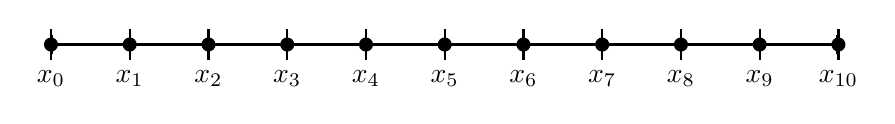
\begin{tikzpicture}
                    \draw[thick,|-|, black] (0,0) -- (10,0);
                    \foreach \j in {0,1,2,3,4,5,6,7,8,9,10}{
                        \draw[black, thick, fill=black] (\j,0) circle(0.075cm);
                        \draw[black, thick] (\j,0.2) -- (\j,-0.2)
                        node[anchor=north]{$x_{\j}$};
                    }
                \end{tikzpicture}
            \end{center}
            How many unknowns are there in this picture?
        \item[(b)] The temperature at each point along the rod is the average of the
            temperatures at the adjacent points.  For example, if we let $T_1$ be the
            temperature at point $x_1$ then
            \[ T_1 = \frac{T_0 + T_2}{2}. \]
            Write a system of equations for each of the unknown temperatures.
        \item[(c)] Solve the system for the temperature at each unknown node.
    \end{enumerate}
\end{problem}
\solution{
    \begin{flalign*}
        T_1 &= \frac{T_0 + T_2}{2} = \frac{100 + T_2}{2} \\
        T_2 &= \frac{T_1 + T_3}{2} \\
        T_3 &= \frac{T_2 + T_4}{2} \\
        T_4 &= \frac{T_3 + T_5}{2} \\
        T_5 &= \frac{T_4 + T_6}{2} \\
        T_6 &= \frac{T_5 + T_7}{2} \\
        T_7 &= \frac{T_6 + T_8}{2} \\
        T_8 &= \frac{T_7 + T_9}{2} \\
        T_9 &= \frac{T_8 + T_{10}}{2} = \frac{T_8}{2} \\
    \end{flalign*}
    Solving this system we get $T_0=100, T_1 = 90, T_2 = 80, T_3 = 70, \cdots, T_10 = 0$.
}


\newpage\section{Additional Exercises}


\begin{problem}
    Now imagine that we are finding the temperature on a flat (2D) metal plate that
    measured 1m
    by 1m (broken into 10cm by 10cm squares).  Extend the idea from Problem
    \ref{prob:heated_rod_lin_alg} to find the temperature at each of
    the interior points if the left and bottom sides are heated to $100^\circ$ and the top
    and right sides are cooled to $0^\circ$.  You will likely need write computer code to
    solve this problem and the best possible output would be a surface (or contour) plot
    showing the temperature.
\end{problem}

\begin{problem}
    Write $d = (3,-5,10)$ as a linear combination of the vectors $a = (-1,0,3)$,
    $b = (0,1,5),$ and $c = (4,-2,0)$. \\
    Choose from:
    \begin{enumerate}
        \item[(a)] $d = -3a - 5b + c$
        \item[(b)] $d = 5a - b + 2c$
        \item[(c)] $d = (10/3)a + (5/2)c$
        \item[(d)] $d$ cannot be written as a linear combination of $a, b$, and $c$.
    \end{enumerate}
\end{problem}
\solution{b}

% \begin{problem}
%     \begin{itemize}
%             \input{ClickerQuestions/LA.00.18.010}
%     \end{itemize}
% \end{problem}
% \solution{
% 2
% }
% 


\begin{problem}
    Consider the system of 2 equations and two unknowns below: 
\[ \left\{ \begin{array}{rl} x+y &= 3 \\ -3x+ky &= 2 \end{array}
    \right. \]
    \begin{enumerate}
        \item[(a)] Determine the value of $k$ for which the system has no solutions.
        \solution{
    \begin{flalign*}
        \left( \begin{array}{cc|c} 1 & 1 & 3 \\ -3 & k & 2 \end{array} \right) &\to
        \left( \begin{array}{cc|c} 1 & 1 & 3 \\ 0 & k+3 & 11 \end{array} \right)
    \end{flalign*}
    If $k=-3$ then the bottom row of the augmented matrix would be read as $0=1$ which is
    always false.
}
    
\item[(b)] If $k$ were to have the value that you indicated  from part (a), what would you
see if you plotted both linear functions on the same coordinate plane?
\solution{
    You will see two parallel lines.
}
\end{enumerate}
\end{problem}

\begin{problem}
Consider the matrix $A$ given below.  It can be shown that $\det(A) = 0$.  For
each of the following true or false questions please circle the correct choice AND provide
a short explanation.
\[ A = \begin{pmatrix} -3 & 0 & 0 & 0 \\ 7 & -1 & 0 & 0 \\ 7 & 1 & 0 & 0 \\ -4 & -8 & 8 &
    1 \end{pmatrix} \quad \text{and we know that} \quad \det(A) = 0 \]
    \begin{enumerate}
        \item[(a)] TRUE or FALSE: \quad The matrix $A$ has an inverse.
    \solution{
        False.  If $\det(A) = 0$ then $A^{-1}$ doesn't exist.
    }

\item[(b)] TRUE or FALSE: \quad Let $B$ be a $4 \times 4$ matrix and let the matrix $C$
    be defined as $C = AB$.  Assume further that $\det(B) = 7$.  Based on all of this, the
    matrix $C$ does not have an inverse.
    \solution{
        True.  $\det(C) = \det(AB) = \det(A) \cdot \det(B) = 0 \cdot 7 = 0$ so $C$ does
        not have an inverse.
    }
\end{enumerate}
\end{problem}

\begin{problem}
    Bonnie and Clyde, two mathematics students from the
    1930's, are solving the same system of three equations in two unknowns.  Bonnie is a more
    visual thinker so she graphs the system.  Her graph is given below on the left.  Clyde
    prefers to follow the mathematical algorithms (sometimes without much thought) and
    arrives at the row-reduced augmented system shown below on the right.  

    \begin{minipage}{0.5\columnwidth}
        \begin{center}
            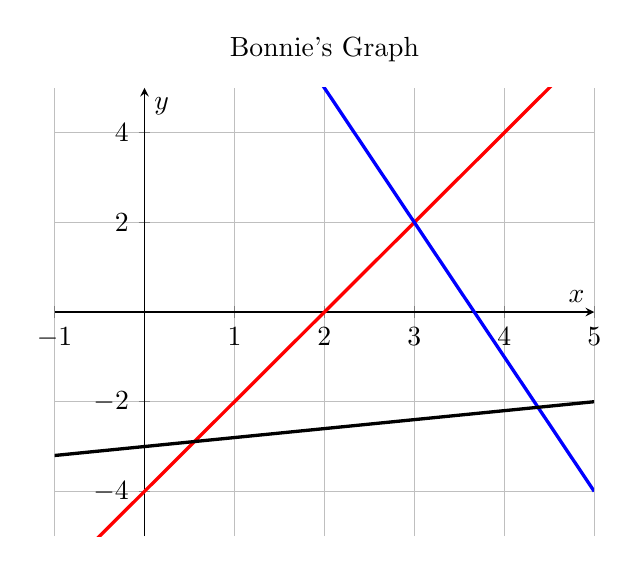
\begin{tikzpicture}
                \begin{axis}[axis lines=center, xlabel={$x$}, ylabel={$y$}, title={Bonnie's
                    Graph}, grid, ymin=-5, ymax=5]
                    \addplot[smooth, red, very thick, domain=-1:5] {2*x-4};
                    \addplot[smooth, blue, very thick, domain=-1:5] {-3*x+11};
                    \addplot[smooth, black, very thick, domain=-1:5] {0.2*x-3};
                \end{axis}
            \end{tikzpicture}
        \end{center}
    \end{minipage}
    \begin{minipage}{0.5\columnwidth}
        \begin{center}
            Clyde's reduced augmented system 
        \end{center}
        \[ \left( \begin{array}{cc|c} 1 & 0 & 3 \\ 0 & 1 & 2 \\ 0 & 0 & 0 \end{array} \right) \]
    \end{minipage}

    \begin{enumerate}
        \item[(a)] What is Bonnie's conclusion about the system of three equations in two
        unknowns?  Explain in a sentence or two.
        \solution{
            Bonnie should conclude that there are no solutions to the system since there
            is no single point where all three lines cross.
        }

    \item[(b)] What is Clyde's conclusion about the system of three equations in two
        unknowns?  Explain in a sentence or two.
        \solution{
            $x=3$ and $y=2$
        }

    \item[(c)] It should be clear (hint hint) that Bonnie and Clyde have different
        solutions to the system of equations.  Give a possible row-reduced matrix for
        Bonnie's graphical solution. 
        \solution{
            \[ \left( \begin{array}{cc|c} 1 & 0 & * \\ 0 & 1 & * \\ 0 & 0 & 1 \end{array} \right) \]
            }
    \end{enumerate}
\end{problem}

\begin{problem}
    For each of the following row reduced systems of equations indicate the number of
    solutions AND
    \begin{itemize}
        \item if there is only 1 solution then given it.  
        \item if there are infinitely many solutions then write an expression that gives
            all of them.
        \item if there are no solutions then explain why not.
    \end{itemize}
    \begin{enumerate}
        \item[(a)] \[ \left( \begin{array}{ccc|c} 1 & 0 & 1 & 4 \\ 0 & 1 & -3 & 2 \\ 0 & 0
                & 0 & 0 \end{array} \right) \]
                \solution{
                    \[ \begin{pmatrix} x_1 \\ x_2 \\ x_3 \end{pmatrix} = \begin{pmatrix} 4
                            \\ 2 \\ 0 \end{pmatrix} + \begin{pmatrix} -1 \\ 3 \\ 1
                            \end{pmatrix} t \quad \text{for} \quad t\in\mathbb{R} \]
                        }
            \item[(b)]  \[ \left( \begin{array}{ccc|c} 1 & 0 & 0 & 4 \\ 0 & 1 & 0 & 2 \\ 0 & 0
                & 1 & 0 \end{array} \right) \]
                \solution{
                    \[ \begin{pmatrix} x_1 \\ x_2 \\ x_3 \end{pmatrix} = \begin{pmatrix} 4
                            \\ 2 \\ 0 \end{pmatrix} \]
                        }
            \item[(c)]  \[ \left( \begin{array}{ccc|c} 1 & 0 & 1 & 4 \\ 0 & 1 & 0 & 2 \\ 0 & 0
                & 0 & 1 \end{array} \right) \]
                \solution{
                    No solution
                }
    \end{enumerate}
\end{problem}

\begin{problem}
    Find a $2 \times 2$ matrix $B$ such that 
    \[ \begin{pmatrix} 1 & 5 \\ 2 & 0 \end{pmatrix} \begin{pmatrix}
            \underline{\hspace{0.25in}} & \underline{\hspace{0.25in}} \\
            \underline{\hspace{0.25in}} & \underline{\hspace{0.25in}} \end{pmatrix} = \begin{pmatrix} 1 & 0 \\ 0 & 1
        \end{pmatrix} \]
\end{problem}
\solution{
    Hint: If you multiply the left-hand matrix by $B$ you get the identity.  What does
    that mean about $B$ and the left-hand matrix?
}

\begin{problem}
    If $A$ and $B$ are $4 \times 4$ matrices with $\det(A) = 2$ and $\det(B) = 5$ then
    evaluate the following.
    \begin{flalign*}
        & \det(AB) = \underline{\hspace{1in}} \\
        & \det(3A) = \underline{\hspace{1in}} \\
        & \det(A^T) = \underline{\hspace{1in}} \\
        & \det(B^{-1}) = \underline{\hspace{1in}} \\
        & \det(B^4) = \underline{\hspace{1in}} \\
    \end{flalign*}
\end{problem}
\solution{
    Hint: Check out the rules of determinants in this chapter.
}
